\documentclass[10pt,a4paper,UTF8]{ctexart}

\linespread{1.5}
\usepackage{geometry}%用于设置上下左右页边距
	\geometry{left=2.5cm,right=2.5cm,top=3.2cm,bottom=2.7cm}
\usepackage{xeCJK,amsmath,paralist,enumerate,booktabs,multirow,graphicx,subfig,setspace,listings,lastpage,hyperref}
\usepackage{amsthm, amssymb, bm, color, framed, graphicx, hyperref, mathrsfs}
\usepackage{mathrsfs}  
	\setlength{\parindent}{2em}
	\lstset{language=Matlab}%
\usepackage{fancyhdr}
\usepackage{graphicx}
\usepackage{subfloat}
\usepackage{listings}
\usepackage{xcolor}
\usepackage{float}
\usepackage{paralist}
\usepackage{setspace}
\usepackage{titlesec}
\usepackage{enumitem}
\usepackage{hyperref}
\usepackage{multirow}
\usepackage{threeparttable}
\usepackage{tcolorbox}
\usepackage{tabularx}
\usepackage{ulem}
\usepackage{multicol}
\usepackage{multirow}
\usepackage{pifont}


\hypersetup{
	colorlinks=true,
	linkcolor=black
}

\setenumerate{partopsep=0pt,topsep=0pt}
\setitemize{itemsep=0pt,partopsep=0pt,topsep=0pt}

\titlespacing*{\section}{0pt}{3pt}{3pt}
\titlespacing*{\subsection}{0pt}{2pt}{2pt}
\titlespacing*{\subsubsection}{0pt}{1pt}{1pt}
\titlespacing*{\paragraph}{0pt}{0pt}{0pt}

\setenumerate{partopsep=-2pt,topsep=-2pt,itemsep=-1pt,leftmargin=2em}
\setitemize{itemsep=-2pt,partopsep=-2pt,topsep=-1pt,leftmargin=2em}

\ctexset{secnumdepth=4,tocdepth=4}
\setlength{\parindent}{2pt}
\setstretch{1.2}


\setCJKmainfont[BoldFont={FZHei-B01},ItalicFont={FZKai-Z03}]{FZShuSong-Z01} 
\setCJKsansfont[BoldFont={FZHei-B01}]{FZKai-Z03} 
\setCJKmonofont[BoldFont={FZHei-B01}]{FZFangSong-Z02}
\setCJKfamilyfont{zhsong}{FZShuSong-Z01} 
\setCJKfamilyfont{zhhei}{FZHei-B01} 
\setCJKfamilyfont{zhkai}[BoldFont={FZHei-B01}]{FZKai-Z03} 
\setCJKfamilyfont{zhfs}[BoldFont={FZHei-B01}]{FZFangSong-Z02} 
\renewcommand*{\songti}{\CJKfamily{zhsong}} 
\renewcommand*{\heiti}{\CJKfamily{zhhei}} 
\renewcommand*{\kaishu}{\CJKfamily{zhkai}} 
\renewcommand*{\fangsong}{\CJKfamily{zhfs}}

\newcommand{\myline}{\underline{\hbox to 10mm{}}}

\definecolor{mKeyword}{RGB}{0,0,255}          % bule
\definecolor{mString}{RGB}{160,32,240}        % purple
\definecolor{mComment}{RGB}{34,139,34}        % green
\definecolor{mNumber}{RGB}{128,128,128} 

\lstdefinestyle {njulisting} {
	basewidth = 0.5 em,
	lineskip = 3 pt,
	basicstyle = \small\ttfamily,
	% keywordstyle = \bfseries,
	commentstyle = \itshape\color{gray}, 
	basicstyle=\small\ttfamily,
	keywordstyle={\color{mKeyword}},     % sets color for keywords
	stringstyle={\color{mString}},       % sets color for strings
	commentstyle={\color{mComment}},     % sets color for comments
	numberstyle=\tiny\color{mNumber},
	numbers = left,
	captionpos = t,
	breaklines = true,
	xleftmargin = 2 em,
	xrightmargin = 2 em,
	frame=tlrb,
	tabsize=4
}

\lstset{
style = njulisting, % 调用上述样式 
flexiblecolumns % 允许调整字符宽度
}


%================= 基本格式预置 ===========================
\usepackage{fancyhdr}
\pagestyle{fancy}
\lhead{操作系统}
\rhead{课后应用题作业1}
\cfoot{\thepage}
\renewcommand{\headrulewidth}{0.4pt}
\renewcommand{\theenumi}{(\arabic{enumi})}
\CTEXsetup[format={\bfseries\zihao{-3}}]{section}
\CTEXsetup[format={\bfseries\zihao{4}}]{subsection}
\CTEXsetup[format={\bfseries\zihao{-4}}]{subsubsection}


\renewcommand{\contentsname}{目录}  

\newcounter{problemname}
%以下为有题目阴影
\definecolor{shadecolor}{RGB}{241, 241, 255}
\newenvironment{problem}{\stepcounter{problemname}\vspace{-0.5em}\begin{shaded}\par\noindent\textbf{\arabic{problemname}. }}{\end{shaded} \vspace{-1em} \par}
%以下为无题目阴影
% \newenvironment{problem}{\stepcounter{problemname}\par\noindent\textbf{\arabic{problemname}. }}{\par}
\newenvironment{solution}{\noindent\textbf{解答:}\\ \indent}{\par}

\begin{document}

\setlength{\parskip}{0.65em}

\begin{center}
\LARGE\textbf{操作系统2022课后应用题作业1}
\end{center}

\begin{problem}
	试述系统调用的实现原理,陷阱机制和绘制系统调用的处理过程,并阐述系统调用的处理逻辑。
\end{problem}

\begin{solution}
	操作系统实现系统调用功能的机制称为系统陷阱或系统异常处理机制,由于系统调用而引起处理器中断的机器指令称为陷入指令(trap),它是非特权指令,在用户态下执行时会产生 CPU 模式切换,即由用户态转换到内核态。每个系统调用都事先规定编号,称为功能号,执行陷入指令时,必须通过某种方式指明对应系统调用的功能号,大多数情况,还应附带有传递给相应服务例程的参数。
	
	系统调用的实现要点包括:(1)编写系统调用服务例程;(2)设计系统调用入口地址表,每个入口地址都指向一个系统调用的服务例程,有些还包含系统调用自带参数的个数;(3)陷阱处理机制,需要开辟现场保护区,以保存发生系统调用时应用程序的处理器现场。

	下图给出了系统调用的处理过程:应用程序执行系统调用,产生中断转向内核态,进入陷阱处理程序,它将按功能号来查询入口地址表,并转至对应服务例程执行,完成后退出中断,返回应用程序断点继续运行。

	\begin{figure}[H]
		\centering
		\vspace{-0.5em}
		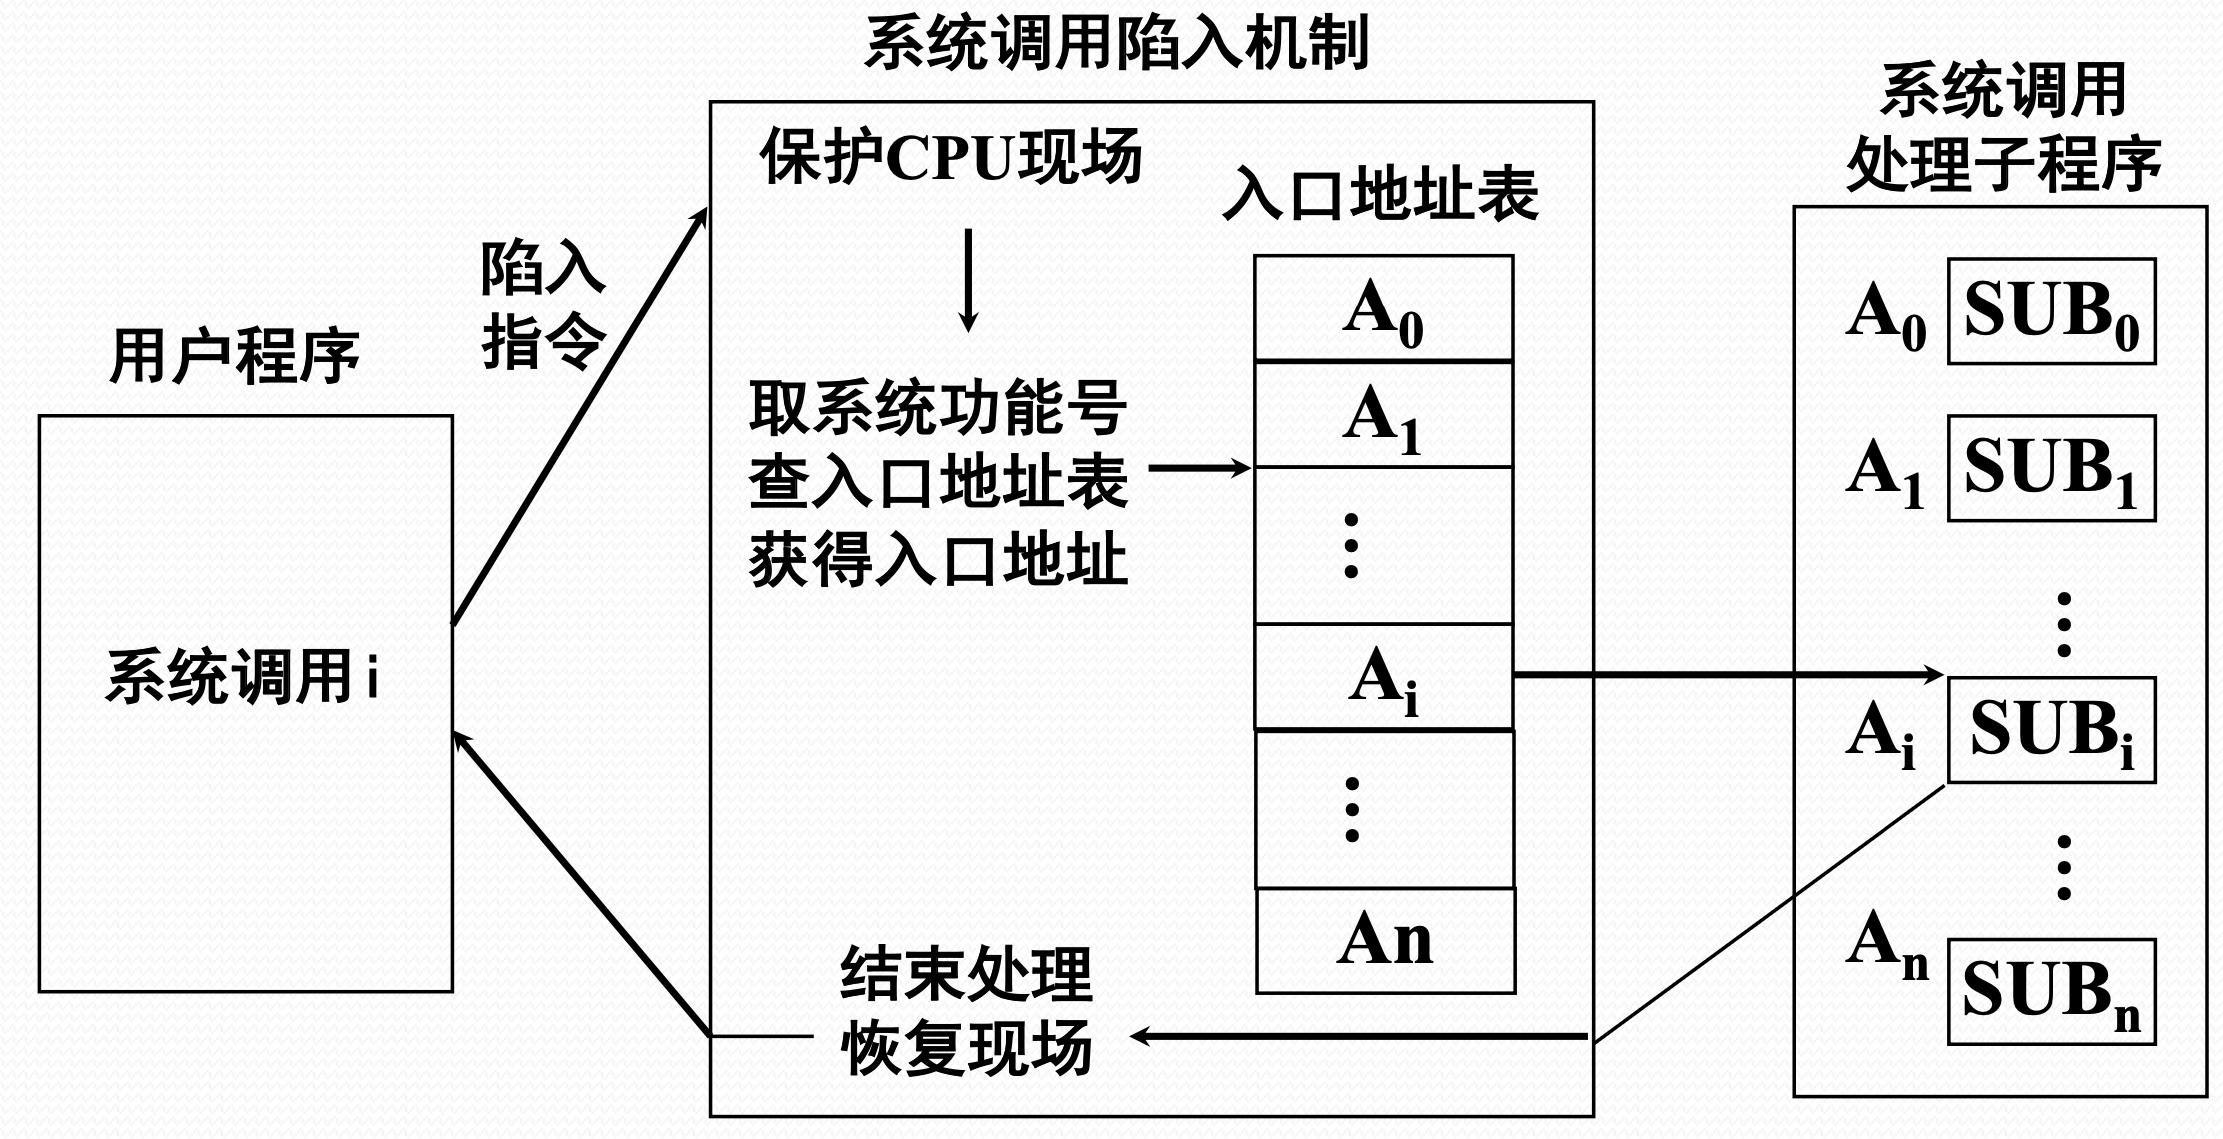
\includegraphics[width=0.6\linewidth]{img/1.png}
		\vspace{-1em}
	\end{figure}


	参数传递是系统调用中需要处理的问题,不同的系统调用要向相应的内核服务例程传递不同参数,反之,执行系统调用的结果也要以参数形式返回给应用程序。实现应用程序和系统调用之间传递参数所采用的方法有:(1)陷入指令自带参数,可以规定陷入指令之后的若干单元存放参数,叫做直接参数;或者在指令之后紧临的单元中存放参数的地址,叫做间接参数,即由间接地址指出参数的存放区;(2)通过 CPU 的通用寄存器传递参数,该方法不适用于传递大量参数,改进方法是在主存的某个区或表中存放参数,将其首地址送入寄存器,实现参数传递;(3)在主存中开辟专用堆栈区传递参数。
\end{solution}


\begin{problem}
	某个计算机系统有一台输入机和一台打印机,现有两道程序投入运行,且程序A先开始运行,程序B后开始运行。程序A的运行轨迹为:计算50ms、打印100ms、再计算50ms、打印100ms,结束。程序B的运行轨迹为:计算50ms、输入80ms、再计算100ms,结束。试说明:
	\begin{enumerate}[label=(\arabic*)]
		\item 两道程序运行时,CPU是否存在空闲等待?若是,在哪段时间内等待?为什么等待?
		\item 程序A、B是否有等待CPU的情况?若有,指出发生等待的时刻。
	\end{enumerate}
\end{problem}

\begin{solution}
	两道程序并发执行过程如下图所示:
	\begin{figure}[H]
		\centering
		\vspace{-0.5em}
		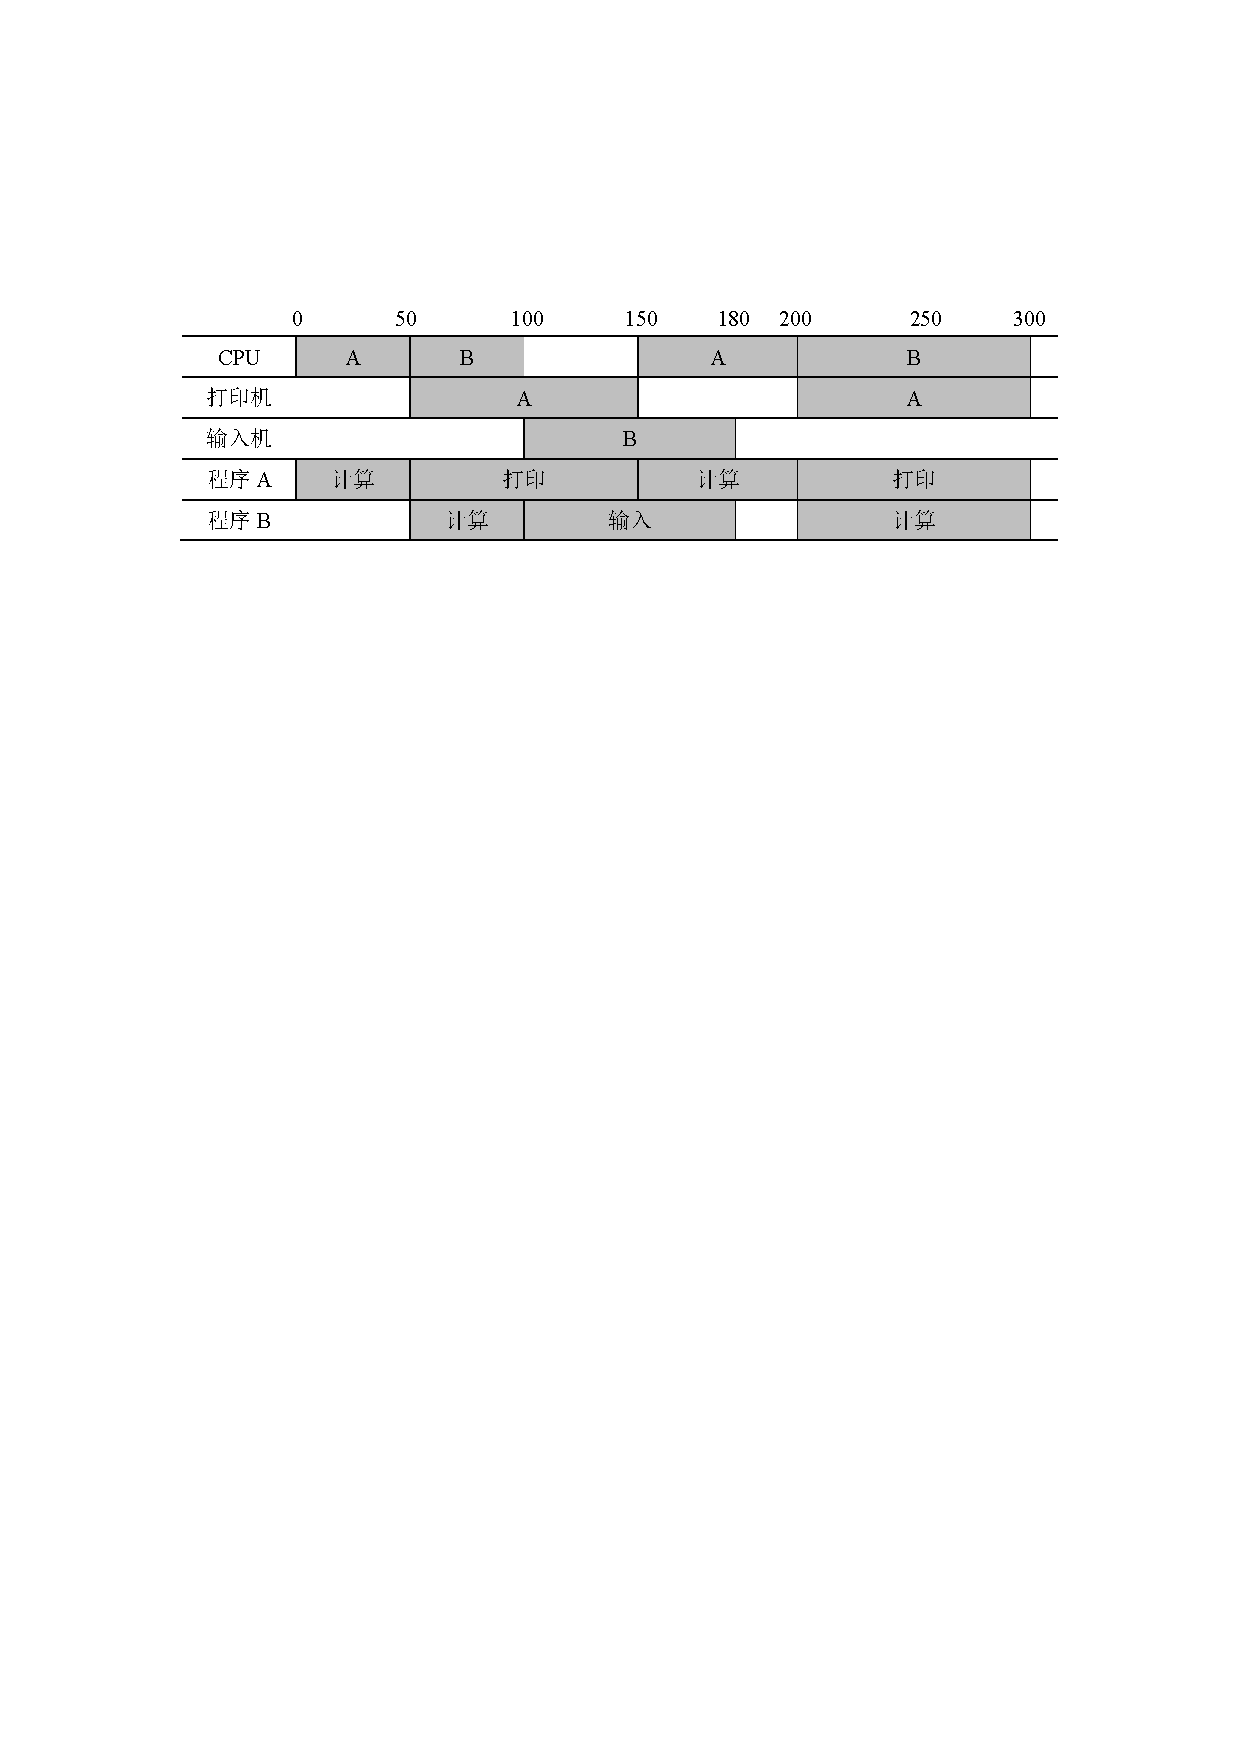
\includegraphics[width=0.65\linewidth]{img/2.pdf}
		\vspace{-1em}
	\end{figure}
	\begin{enumerate}[label=(\arabic*)]
		\item CPU存在空闲等待,空闲等待时间为100ms到150ms,此时A在占用打印机,B在占用输入机,均不需要占用CPU计算,因此CPU处于等待状态。
		\item 程序A不存在等待CPU的情况;程序B存在,发生等待的时刻为0到50ms以及180ms到200ms。
	\end{enumerate}
\end{solution}


\begin{problem}
	若内存中有3道程序A、B、C,按照A、B、C的优先次序运行。各程序的计算轨迹为:
	\begin{enumerate}[label=]
		\item A:计算(20ms),I/O\;(30ms),计算(10ms)
		\item B:计算(40ms),I/O\;(20ms),计算(10ms) 
		\item C:计算(10ms),I/O\;(30ms),计算(20ms)
	\end{enumerate}
	如果3道程序都使用相同的设备进行I/O操作(即程序以串行方式使用设备,调度开销忽略不计),试分别画出(1)单道和(2)多道运行的时间关系图。在两种情况下,CPU的平均利用率各是多少?
\end{problem}
	
\begin{solution}
	(1)单道运行的时间关系图如下,CPU平均利用率为$(20+10+40+10+10+20)\div 190=57.89\%$。
	\begin{figure}[H]
		\centering
		\vspace{-0.5em}
		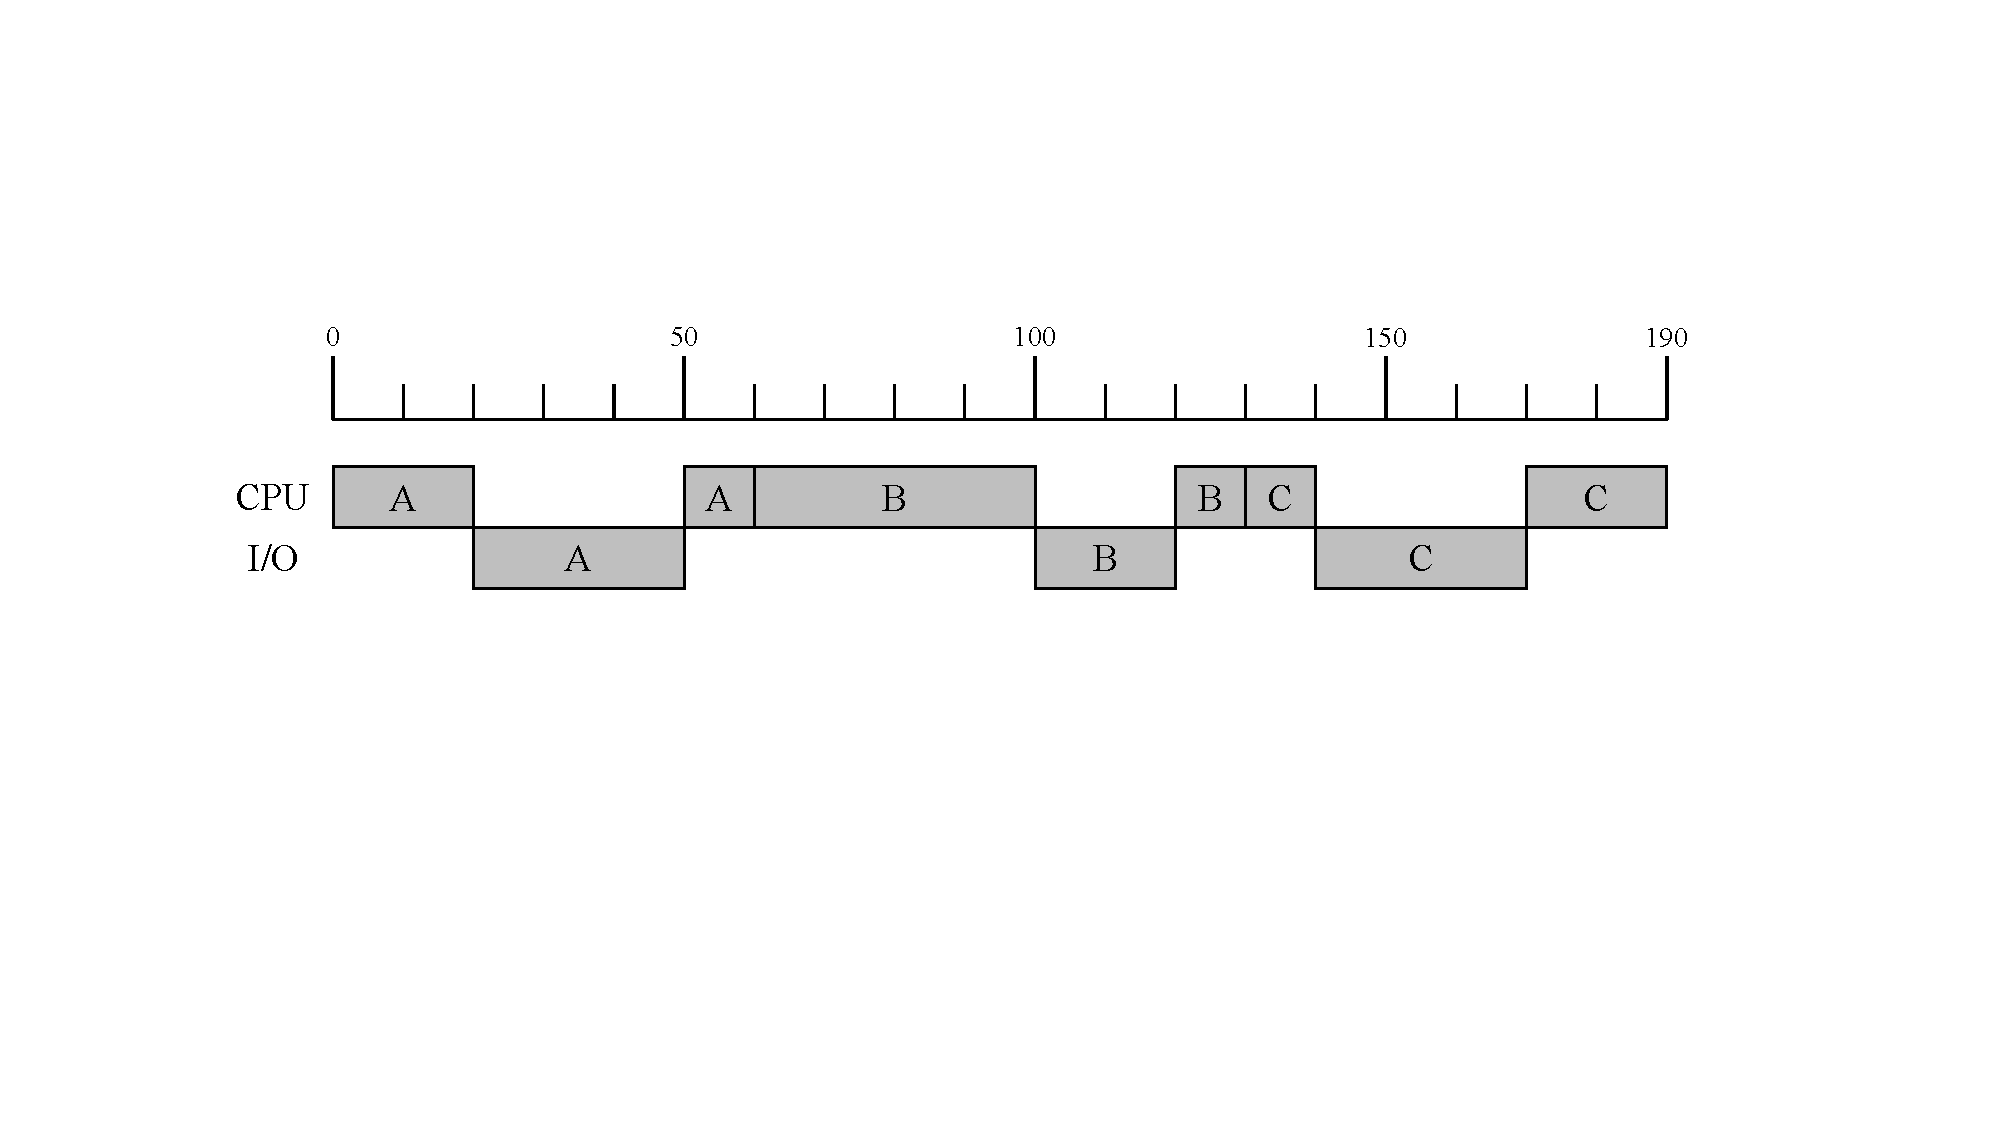
\includegraphics[width=0.8\linewidth]{img/3.1.pdf}
		\vspace{-1em}
	\end{figure}

	(2)多道运行的时间关系图如下,CPU平均利用率为$(20+30+10+10+10+10+20)\div 140=78.57\%$。
	\begin{figure}[H]
		\centering
		\vspace{-0.5em}
		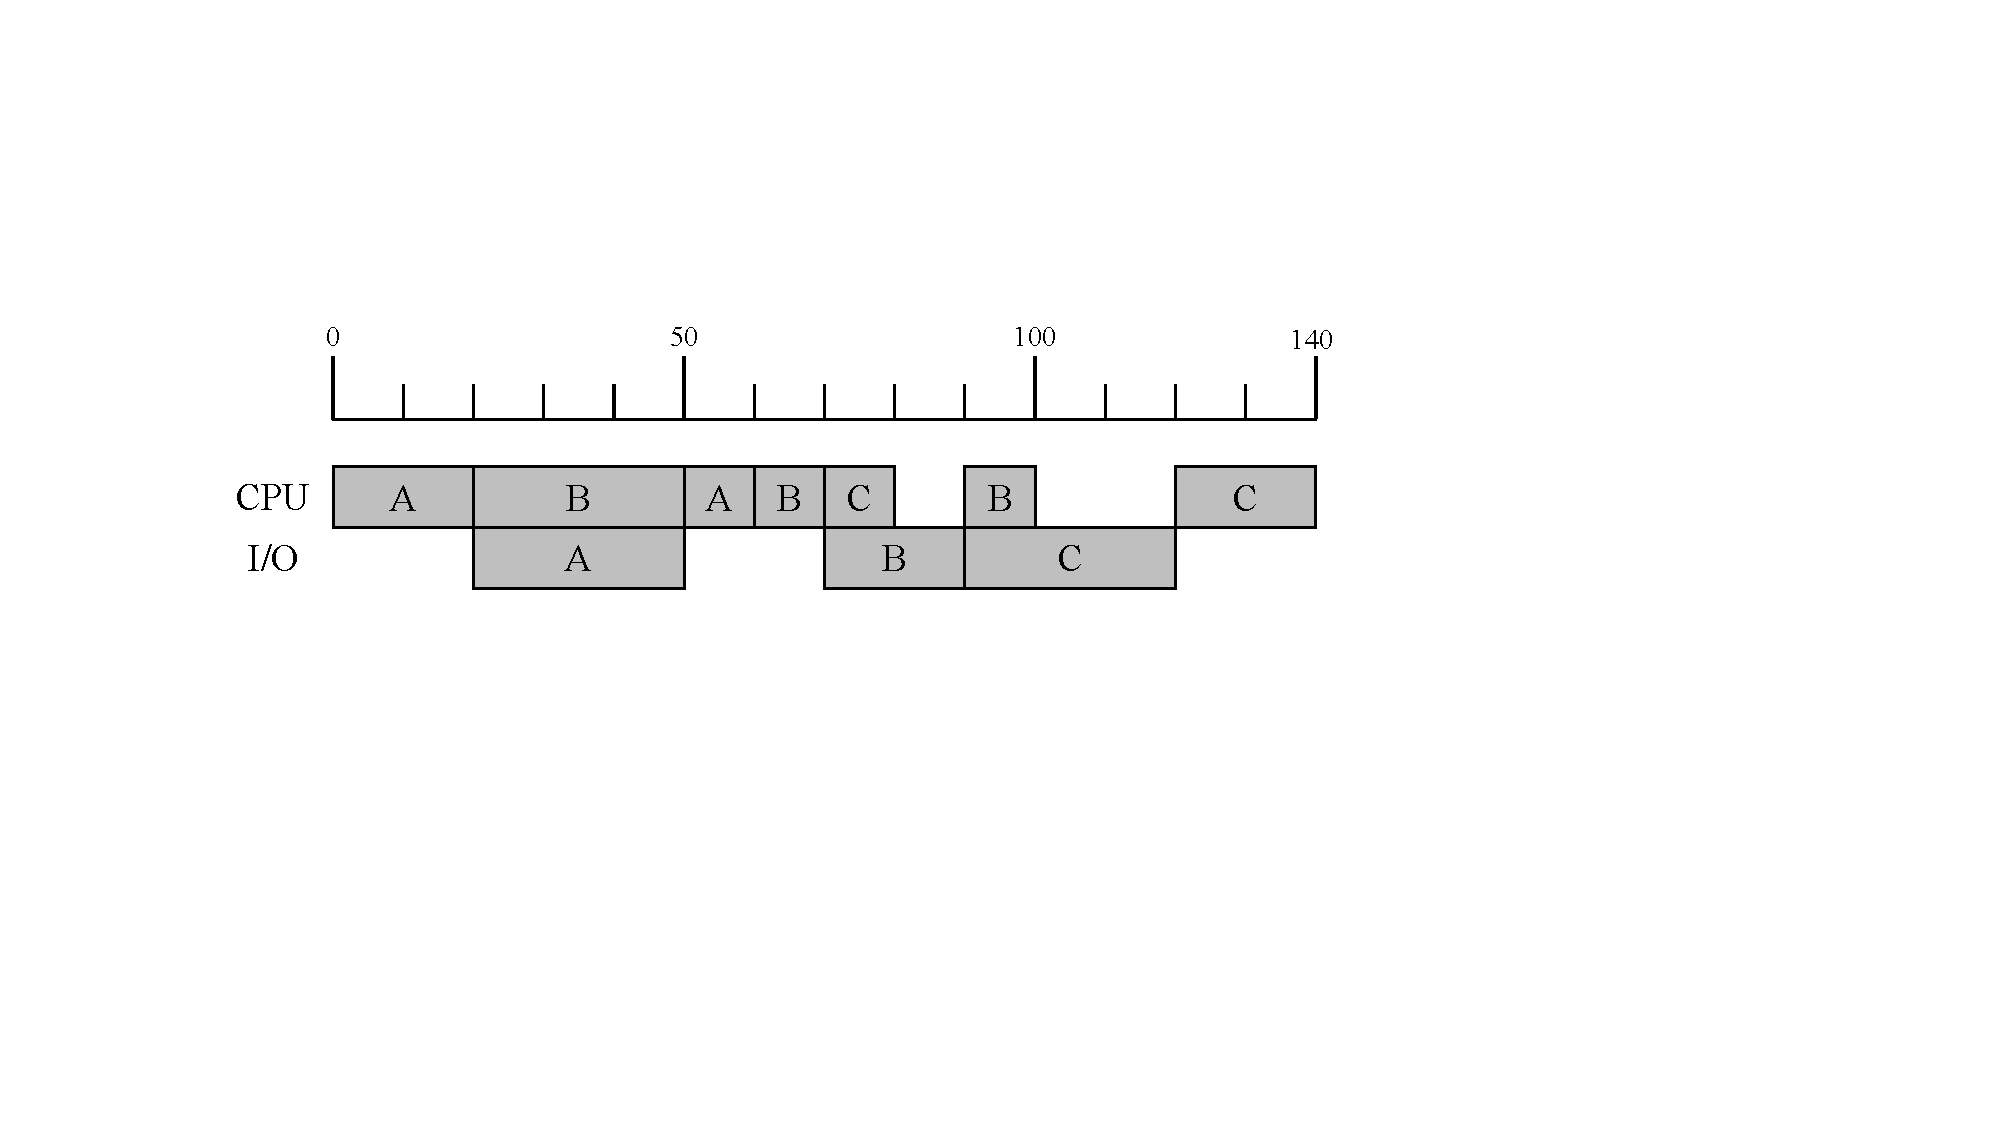
\includegraphics[width=0.65\linewidth]{img/3.2.pdf}
		\vspace{-1em}
	\end{figure}
\end{solution}


\begin{problem}
	在单机系统中,有CPU和两个设备DEV1、DEV2,它们能够同时工作。现有两个程序A、B同时到达,程序B的优先级高于程序A,但当程序A占用CPU时,程序B不能抢占。程序在CPU与IO设备之间的切换开销忽略不计。如果这两个程序使用CPU、DEV1、DEV2的顺序和时间如下表所示。
	\begin{figure}[H]
		\centering
		\vspace{-0.5em}
		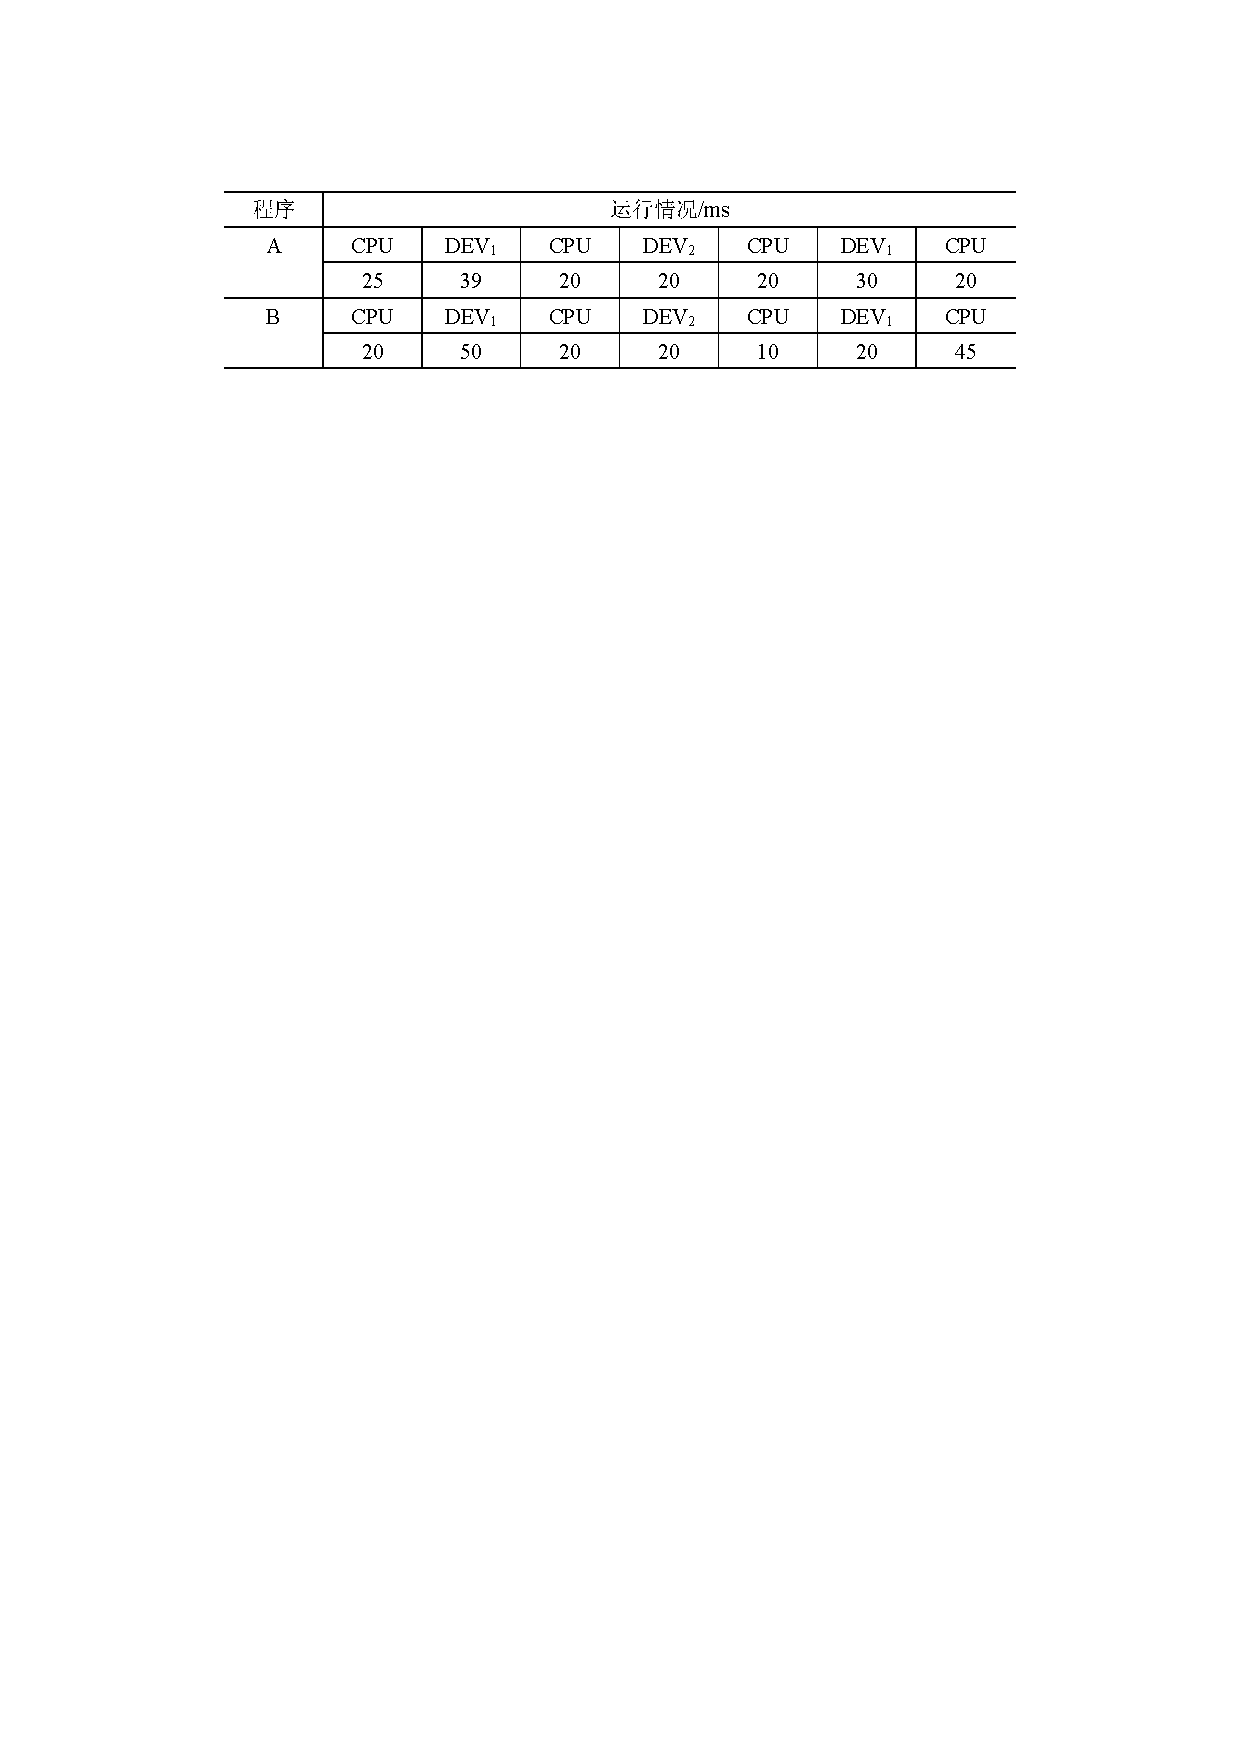
\includegraphics[width=0.85\linewidth]{img/4.1.pdf}
		\vspace{-1em}
	\end{figure}
	试解答下列问题:
	\begin{enumerate}[label=(\arabic*)]
		\item 哪个程序先结束?
		\item 程序全部执行结束需要多长时间?
		\item 程序全部执行完毕时,CPU的利用率是多少?
		\item 程序A等待CPU的累计时间是多少?
		\item 程序B等待CPU的累计时间是多少?
	\end{enumerate}
\end{problem}

\begin{solution}
	程序执行过程如下图所示:
	\begin{figure}[H]
		\centering
		\vspace{-0.5em}
		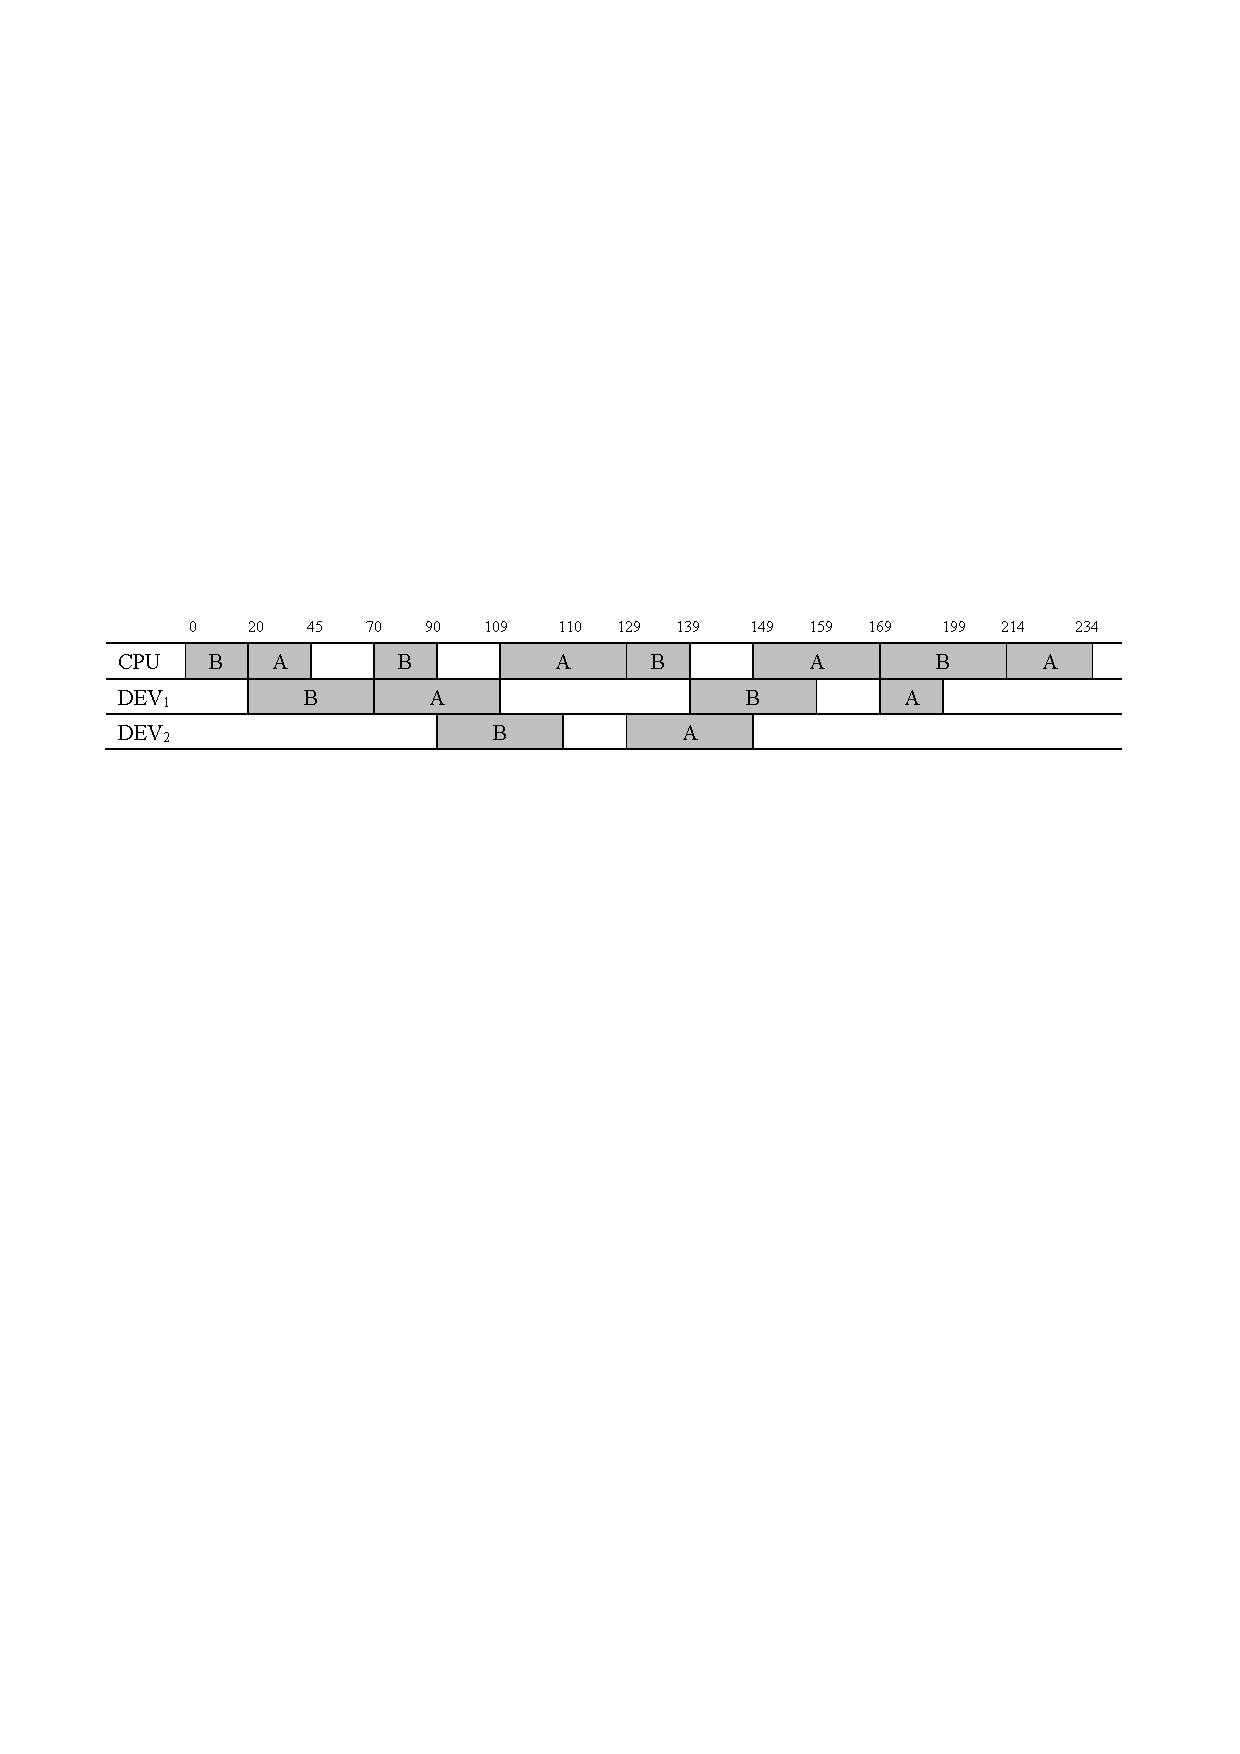
\includegraphics[width=\linewidth]{img/4.2.pdf}
		\vspace{-1em}
	\end{figure}
	\begin{enumerate}[label=(\arabic*)]
		\item B先结束;
		\item 如上图所示,程序全部执行结束需要234ms;
		\item CPU的利用率$(20+25+20+20+10+20+45+20)\div 234=76.92\%$;
		\item 程序A等待CPU的时间分别为$0\sim 20$ms,$199 \sim 214$ms,累计时间为35ms;
		\item 程序B等待CPU到时间分别为$110\sim 129$ms,$159\sim 169$ms,累计时间为29ms。
	\end{enumerate}
\end{solution}


\begin{problem}
	在一个只支持四道程序同时运行的多道程序系统中,若在一段时间内先后到达6个作业,其提交时刻和估计运行时间由下表给出。
	\begin{table}[H]
		\centering
		\vspace{-0.5em}
		\begin{tabular}{|c|c|c|}
		\hline
		作业 & 提交时刻 & 估计运行时间/min \\ \hline
		1  & 8:00 & 60         \\ \hline
		2  & 8:20 & 35         \\ \hline
		3  & 8:25 & 20         \\ \hline
		4  & 8:30 & 25         \\ \hline
		5  & 8:35 & 5          \\ \hline
		6  & 8:40 & 10         \\ \hline
		\end{tabular}
		\vspace{-1.5em}
	\end{table}
	系统采用SRTF调度算法,作业被调度进入系统后中途不会退出,但作业运行时可被剩余时间更短的作业所抢占。
	\begin{enumerate}[label=(\arabic*)]
		\item 分别给出6个作业的开始执行时间、作业完成时间、作业周转时间。
		\item 计算平均作业周转时间。
	\end{enumerate}
\end{problem}

\begin{solution}
	作业调度执行过程如下:
	\begin{figure}[H]
		\centering
		\vspace{-0.5em}
		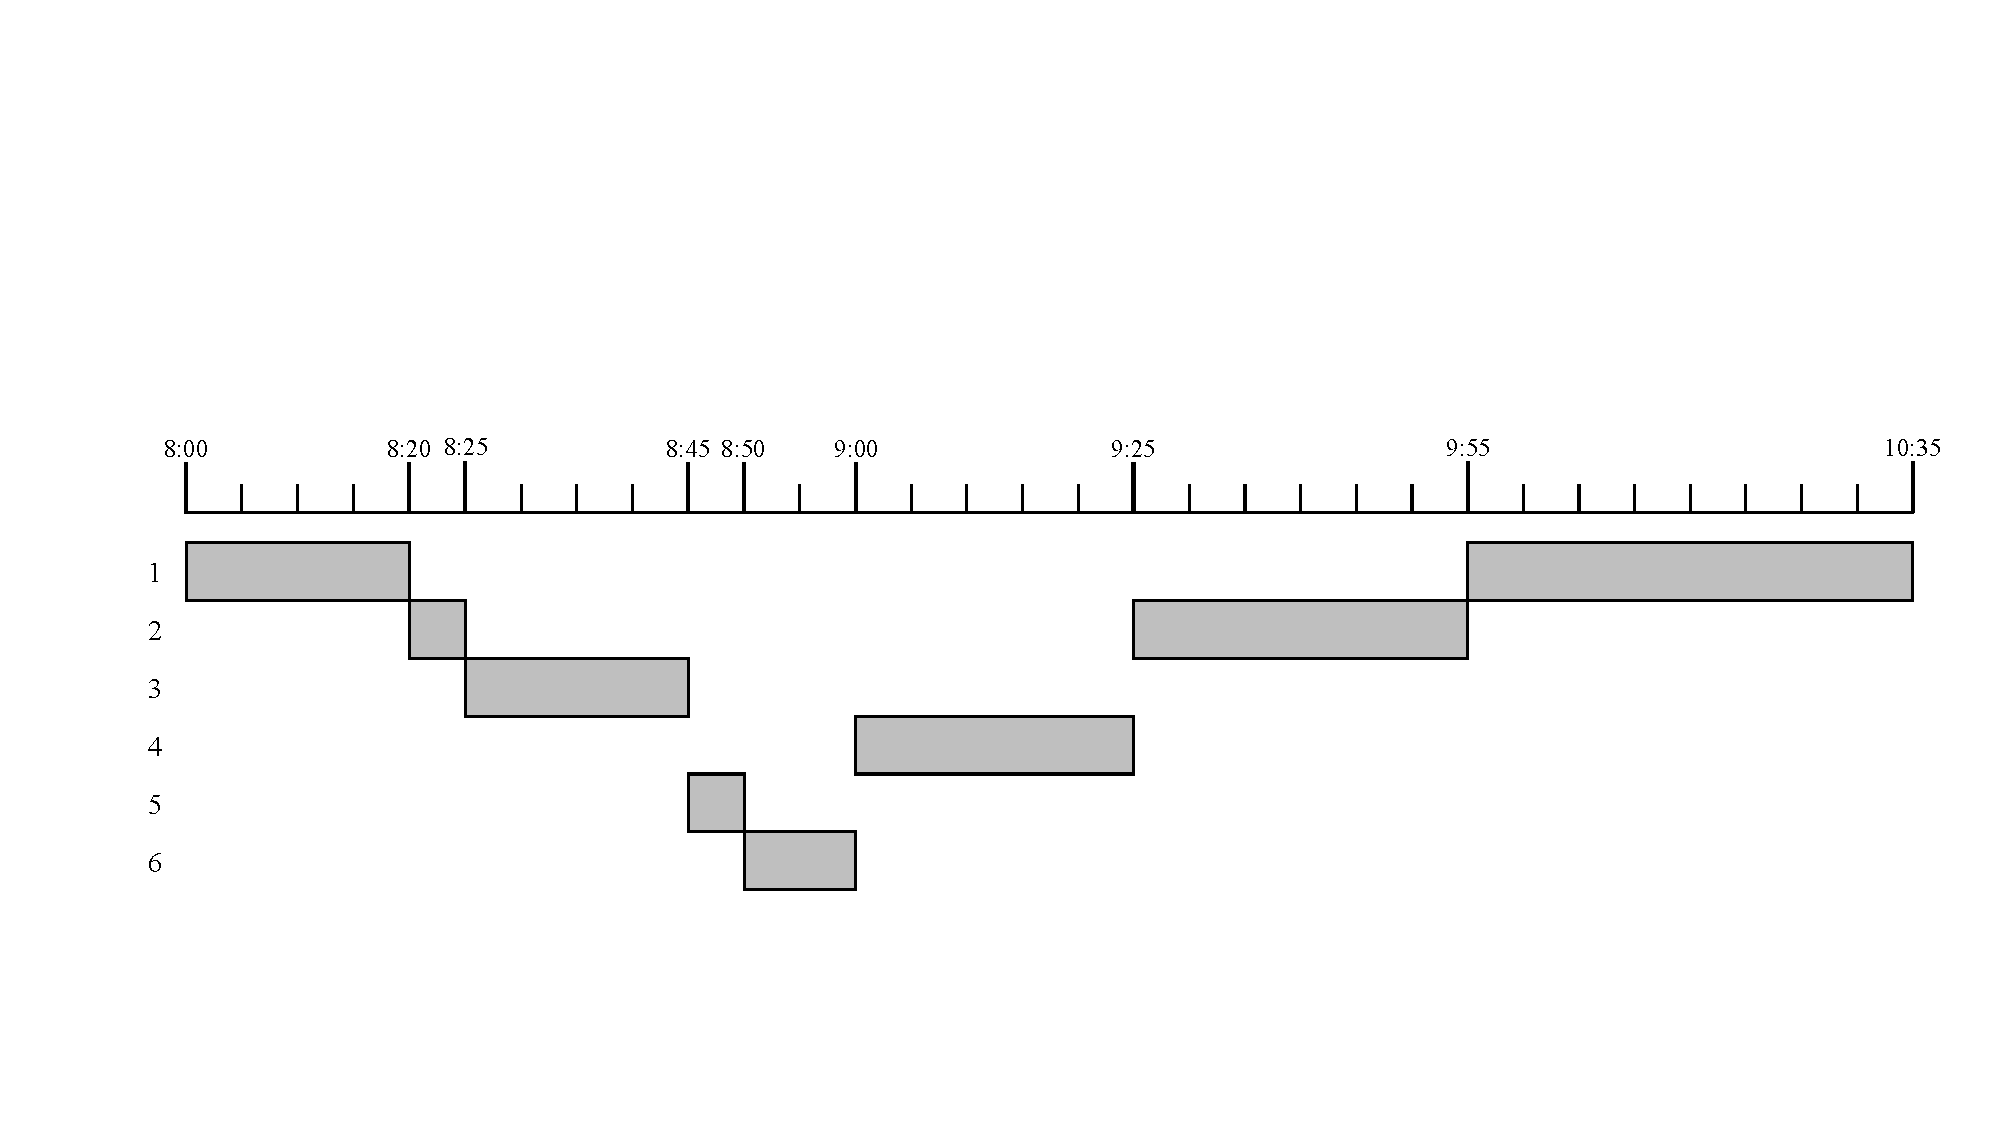
\includegraphics[width=\linewidth]{img/5.pdf}
		\vspace{-1em}
	\end{figure}
	\begin{itemize}
		\item 8:20时,作业1剩余时间为40min,作业2剩余时间为35min,执行作业2;
		\item 8:25时,作业1剩余时间为40min,作业2剩余时间为30min,作业3剩余时间为20min,执行作业3;
		\item 8:30时,作业1剩余时间为40min,作业2剩余时间为30min,作业3剩余时间为15min,作业4剩余时间为25min,执行作业3。由于只支持四道程序,之后的作业无法进入内存,直至作业3执行完;
		\item 8:45时,作业3执行完,作业5进入内存,此时作业1剩余时间为40min,作业2剩余时间为30min,作业4剩余时间为25min,作业5剩余时间为5min,执行作业5;
		\item 8:50时,作业5执行完,作业6进入内存,此时作业1剩余时间为40min,作业2剩余时间为30min,作业4剩余时间为25min,作业6剩余时间为10min,执行作业6;
		\item 9:00时,作业6执行完,此时作业1剩余时间为40min,作业2剩余时间为30min,作业4剩余时间为25min,执行作业4;
		\item 9:25时,作业4执行完,此时作业1剩余时间为40min,作业2剩余时间为30min,执行作业2;
		\item 9:55时,作业2执行完,执行作业1;
		\item 10:35时,作业1执行完,全部作业执行完成。	
	\end{itemize}

	(1)如下表所示
	\begin{table}[H]
		\centering
		\vspace{-0.5em}
		\begin{tabular}{|c|c|c|c|c|}
		\hline
		作业号 & 提交时刻 & 开始执行时刻 & 作业完成时刻 & \begin{tabular}[c]{@{}c@{}}作业周转时间\\ (单位:分钟)\end{tabular} \\ \hline
		1   & 8:00 & 8:00   & 10:35  & 155                                                      \\ \hline
		2   & 8:20 & 8:20   & 9:55   & 95                                                       \\ \hline
		3   & 8:25 & 8:25   & 8:45   & 20                                                       \\ \hline
		4   & 8:30 & 9:00   & 9:25   & 55                                                       \\ \hline
		5   & 8:35 & 8:45   & 8:50   & 15                                                       \\ \hline
		6   & 8:40 & 8:50   & 9:00   & 20                                                       \\ \hline
		\end{tabular}
		\vspace{-1em}
	\end{table}
	(2)平均作业周转时间为$(155+95+20+55+15+20)\mathrm{min}\div 6=60\mathrm{min}$。
\end{solution}


\begin{problem}
	设有4个进程$P_1$、$P_2$、$P_3$、$P_4$,它们到达就绪队列的时刻、运行时间及优先级(优先数越大优先级越高)如下表:
	\begin{table}[H]
		\centering
		\vspace{-0.5em}
		\begin{tabular}{|c|c|c|c|}
		\hline
		进程 & 到达就绪队列的时刻 & 运行时间/ms & 优先级 \\ \hline
		$P_1$ & 0         & 9       & 1   \\ \hline
		$P_2$ & 1         & 4       & 3   \\ \hline
		$P_3$ & 2.5       & 8       & 2   \\ \hline
		$P_4$ & 3.5       & 10      & 4   \\ \hline
		\end{tabular}
		\vspace{-1em}
	\end{table}
	\begin{enumerate}[label=(\arabic*)]
		\item 若采用抢占式优先数调度算法(抢占的时间点为高优先级进程达到就绪队列的时刻),试给出各个进程的调度次序以及进程的平均周转时间和平均等待时间。
		\item 若采用时间片轮换调度算法,且时间片长度取2ms,试给出各个进程的调度次序以及进程的平均周转时间和平均等待时间。
	\end{enumerate}
\end{problem}

\begin{solution}
	(1)进程执行过程如下:
	\begin{figure}[H]
		\centering
		\vspace{-0.5em}
		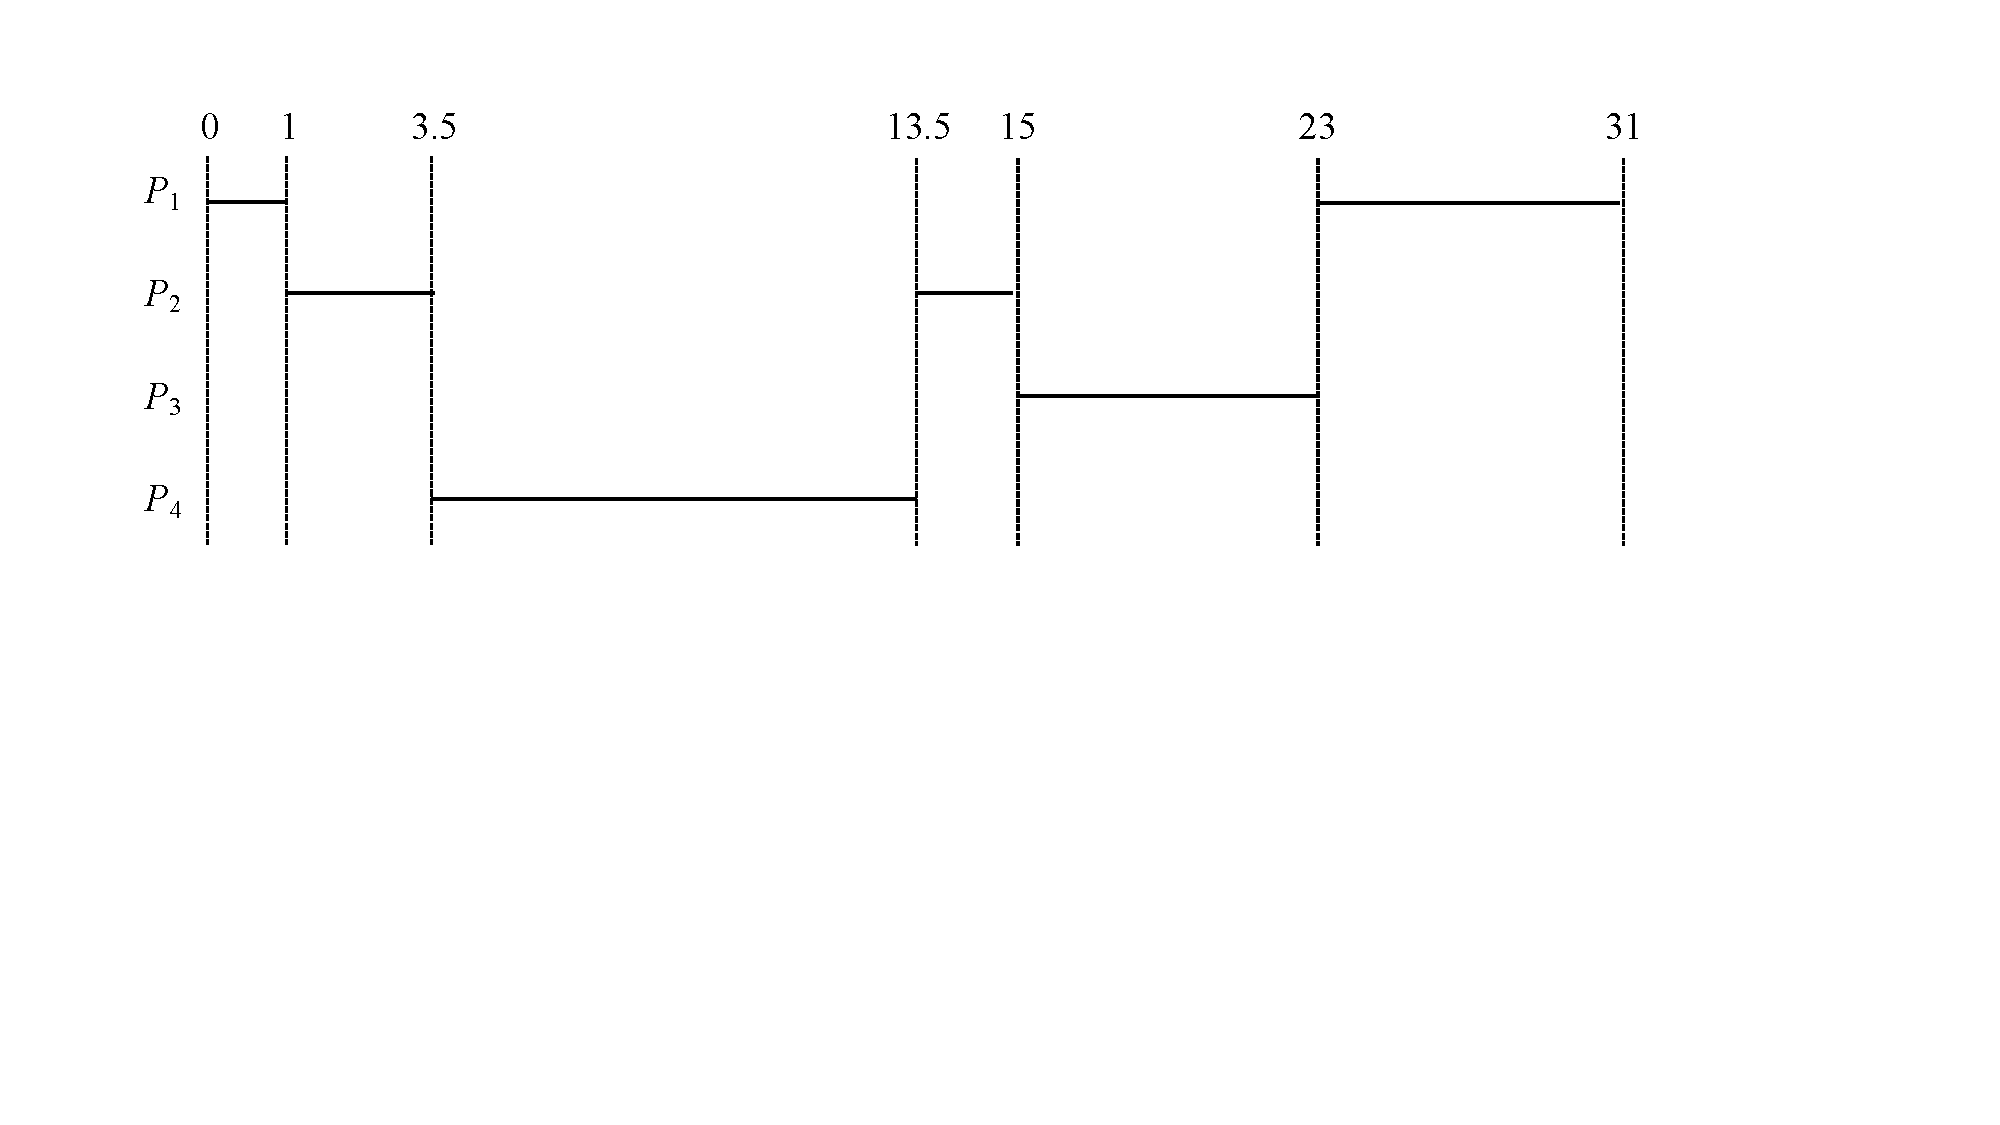
\includegraphics[width=0.6\linewidth]{img/6.1.pdf}
		\vspace{-1em}
	\end{figure}
	进程调度次序为:$P_1$、$P_2$、$P_4$、$P_2$、$P_3$、$P_1$
	
	平均周转时间为:$(31+14+20.5+10)\mathrm{ms} \div 4=18.875\mathrm{ms}$
	
	平均等待时间为:$(22+10+12.5+0)\mathrm{ms} \div 4=11.125\mathrm{ms}$

	\begin{table}[H]
		\vspace{-0.5em}
		\centering
		\begin{tabular}{|c|c|c|c|c|c|}
		\hline
		进程 & 到达就绪队列的时刻 & 运行时间/ms & 完成时刻 & 周转时间/ms & 等待时间/ms \\ \hline
		$P_1$ & 0         & 9       & 31   & 31      & 22      \\ \hline
		$P_2$ & 1         & 4       & 15   & 14      & 10      \\ \hline
		$P_3$ & 2.5       & 8       & 23   & 20.5    & 12.5    \\ \hline
		$P_4$ & 3.5       & 10      & 13.5 & 10      & 0       \\ \hline
		\end{tabular}
		\vspace{-1.5em}
	\end{table}

	(2)进程执行过程如下:

	\begin{figure}[H]
		\centering
		\vspace{-0.5em}
		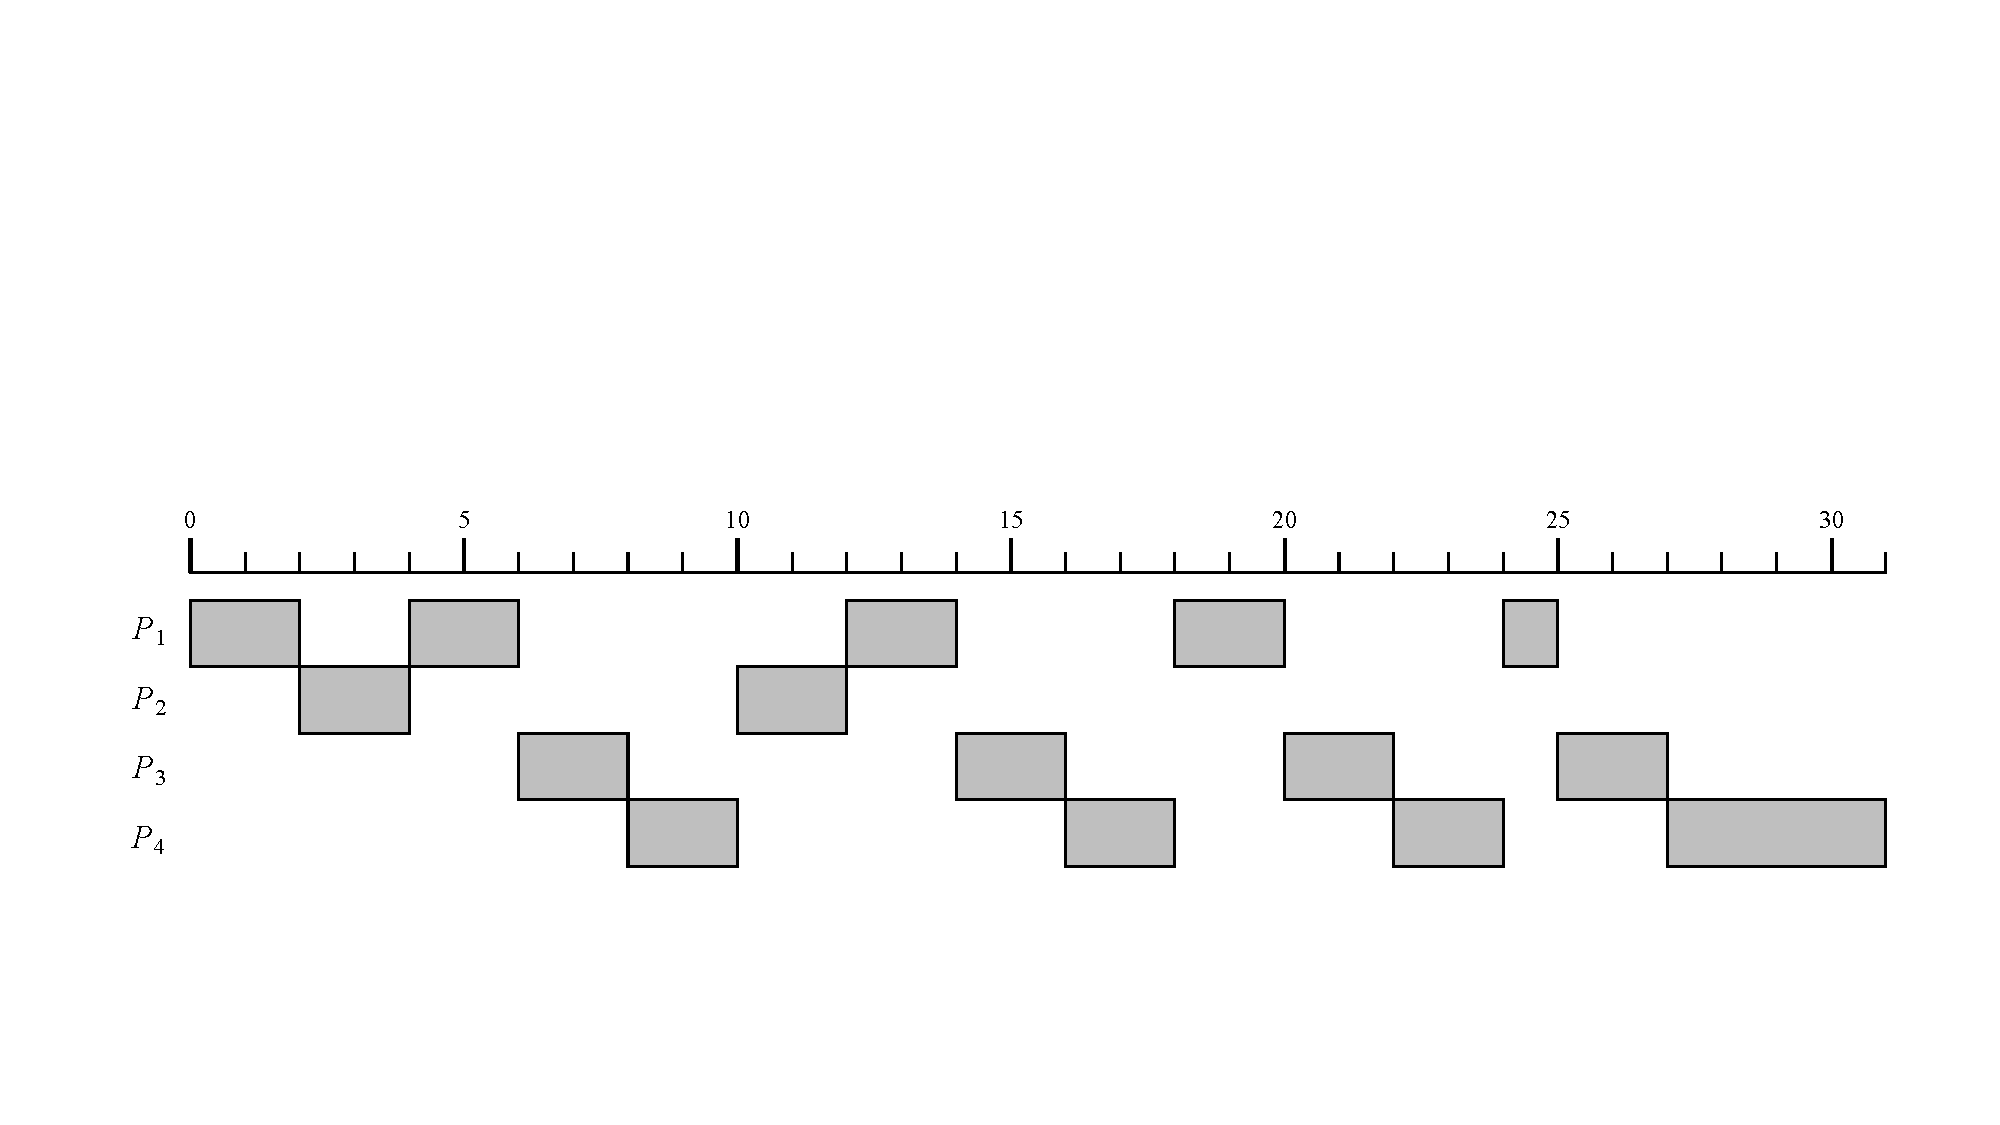
\includegraphics[width=0.85\linewidth]{img/6.2.pdf}
		\vspace{-1em}
	\end{figure}

	进程调度次序为$P_1$、$P_2$、$P_1$、$P_3$、$P_4$、$P_2$、$P_1$、$P_3$、$P_4$、$P_1$、$P_3$、$P_4$、$P_1$、$P_3$、$P_4$
	
	平均周转时间为:$(25+11+24.5+27.5)\mathrm{ms} \div 4=22\mathrm{ms}$
	
	平均等待时间为:$(16+7+16.5+17.5)\mathrm{ms} \div =14.25\mathrm{ms}$

	\begin{table}[H]
		\vspace{-0.5em}
		\centering
		\begin{tabular}{|c|c|c|c|c|c|}
		\hline
		进程 & 到达就绪队列的时刻 & 运行时间/ms & 完成时刻 & 周转时间/ms & 等待时间/ms \\ \hline
		$P_1$ & 0         & 9       & 25   & 25      & 16     \\ \hline
		$P_2$ & 1         & 4       & 12   & 11      & 7      \\ \hline
		$P_3$ & 2.5       & 8       & 27   & 24.5    & 16.5   \\ \hline
		$P_4$ & 3.5       & 10      & 31   & 27.5    & 17.5   \\ \hline
		\end{tabular}
		\vspace{-1em}
	\end{table}
\end{solution}


\begin{problem}
	某一页式存储管理系统,假设其页表全部存放在内存中。
	\begin{enumerate}[label=(\arabic*)]
		\item 若访问内存的时间为120ns,那么访问一个数据的时间是多少?
		\item 若增加一个快表,无论命中与否均需20ns的开销,假设快表的命中率为80\%,则此时访问一个数据的时间是多少?
	\end{enumerate}
\end{problem}

\begin{solution}
	\vspace{-1.5em}
	\begin{enumerate}[label=(\arabic*)]
		\item $120\mathrm{ns}\times 2 = 240\mathrm{ns}$
		\item $80\%\times (120\mathrm{ns}+20\mathrm{ns})+20\%\times (120\mathrm{ns} +120 \mathrm{ns}+20 \mathrm{ns})=164\mathrm{ns}$
	\end{enumerate}
\end{solution}


\begin{problem}
	在一页式存储管理系统中,逻辑地址长度为16位,页面大小为4096B,已知第0、1、2页依次存放在第10、12、14号物理块中,现有逻辑地址2F6AH,请问其相应的物理地址是多少?(地址以十六进制表示)
\end{problem}

\begin{solution}
	由于逻辑地址长度为16位,页面大小为4096B,所以后12位表示页内偏移量,前4位表示逻辑页号,对于逻辑地址2F6AH,其逻辑页号为2,对应物理页号为14,所以该逻辑地址的物理地址是EF6AH。
\end{solution}


\begin{problem}
	假设一个物理存储器有4个页框,一个程序运行的页面走向是:$1-2-3-1-4-5-1-2-1-4-5-3-4-5$。假定所有页框最初都是空的,分别使用OPT、FIFO、LRU、CLOCK、MIN(滑动窗口$\tau=3$)、WS(工作集窗口尺寸$\Delta=2$)算法,计算访问过程中所发生的缺页中断次数和缺页中断率。
\end{problem}

\begin{solution}
	(1)最优置换算法OPT:缺页6次,缺页中断率$=6\div 14=42.86\%$。
	\begin{table}[H]
		\vspace{-0.5em}
		\centering
		\begin{tabular}{|c|c|c|c|c|c|c|c|c|c|c|c|c|c|c|}
		\hline
		页面序列 & 1 & 2 & 3 & 1 & 4 & 5 & 1 & 2 & 1 & 4 & 5 & 3 & 4 & 5 \\ \hline
		页框1  & 1 & 1 & 1 & 1 & 1 & 1 & 1 & 1 & 1 & 1 & 1 & 3 & 3 & 3 \\ \hline
		页框2  &   & 2 & 2 & 2 & 2 & 2 & 2 & 2 & 2 & 2 & 2 & 2 & 2 & 2 \\ \hline
		页框3  &   &   & 3 & 3 & 3 & 5 & 5 & 5 & 5 & 5 & 5 & 5 & 5 & 5 \\ \hline
		页框4  &   &   &   &   & 4 & 4 & 4 & 4 & 4 & 4 & 4 & 4 & 4 & 4 \\ \hline
		缺页标记 & F & F & F &   & F & F &   &   &   &   &   & F &   &   \\ \hline
		\end{tabular}
		\vspace{-1em}
	\end{table}

	(2)先进先出算法FIFO:缺页10次,缺页中断率$=10\div 14=71.43\%$。
	\begin{table}[H]
		\vspace{-0.5em}
		\centering
		\begin{tabular}{|c|c|c|c|c|c|c|c|c|c|c|c|c|c|c|}
		\hline
		页面序列 & 1 & 2 & 3 & 1 & 4 & 5 & 1 & 2 & 1 & 4 & 5 & 3 & 4 & 5 \\ \hline
		页框1  & 1 & 1 & 1 & 1 & 1 & 5 & 5 & 5 & 5 & 5 & 5 & 5 & 4 & 4 \\ \hline
		页框2  &   & 2 & 2 & 2 & 2 & 2 & 1 & 1 & 1 & 1 & 1 & 1 & 1 & 5 \\ \hline
		页框3  &   &   & 3 & 3 & 3 & 3 & 3 & 2 & 2 & 2 & 2 & 2 & 2 & 2 \\ \hline
		页框4  &   &   &   &   & 4 & 4 & 4 & 4 & 4 & 4 & 4 & 3 & 3 & 3 \\ \hline
		缺页标记 & F & F & F &   & F & F & F & F &   &   &   & F & F & F \\ \hline
		\end{tabular}
		\vspace{-1em}
	\end{table}

	(3)最近最少使用算法LRU:缺页7次,缺页中断率$=7\div 14=50\%$。
	\begin{table}[H]
		\vspace{-0.5em}
		\centering
		\begin{tabular}{|c|c|c|c|c|c|c|c|c|c|c|c|c|c|c|}
		\hline
		页面序列 & 1 & 2 & 3 & 1 & 4 & 5 & 1 & 2 & 1 & 4 & 5 & 3 & 4 & 5 \\ \hline
		页框1  & 1 & 1 & 1 & 1 & 1 & 1 & 1 & 1 & 1 & 1 & 1 & 1 & 1 & 1 \\ \hline
		页框2  &   & 2 & 2 & 2 & 2 & 5 & 5 & 5 & 5 & 5 & 5 & 5 & 5 & 5 \\ \hline
		页框3  &   &   & 3 & 3 & 3 & 3 & 3 & 2 & 2 & 2 & 2 & 3 & 3 & 3 \\ \hline
		页框4  &   &   &   &   & 4 & 4 & 4 & 4 & 4 & 4 & 4 & 4 & 4 & 4 \\ \hline
		缺页标记 & F & F & F &   & F & F &   & F &   &   &   & F &   &   \\ \hline
		\end{tabular}
		\vspace{-1em}
	\end{table}

	(4)Clock调度算法:缺页10次,缺页中断率$=10\div 14=71.43\%$。
	\begin{table}[H]
		\vspace{-0.5em}
		\centering
		\begin{tabular}{|c|c|c|c|c|c|c|c|c|c|c|c|c|c|c|}
		\hline
		页面序列 & 1  & 2  & 3  & 1  & 4   & 5  & 1  & 2  & 1  & 4   & 5   & 3   & 4  & 5  \\ \hline
		页框1  & 1* & 1* & 1* & 1* & →1* & 5* & 5* & 5* & 5* & 5*  & 5*  & →5* & 4* & 4* \\ \hline
		页框2  & →  & 2* & 2* & 2* & 2*  & →2 & 1* & 1* & 1* & 1*  & 1*  & 1*  & →1 & 5* \\ \hline
		页框3  &    & →  & 3* & 3* & 3*  & 3  & →3 & 2* & 2* & 2*  & 2*  & 2*  & 2  & →2 \\ \hline
		页框4  &    &    & →  & →  & 4*  & 4  & 4  & →4 & →4 & →4* & →4* & 3*  & 3  & 3  \\ \hline
		缺页标记 & F  & F  & F  &    & F   & F  & F  & F  &    &     &     & F   & F  & F  \\ \hline
		\end{tabular}
		\vspace{-1em}
	\end{table}

	(5)MIN(滑动窗口$\tau=3$):缺页9次,缺页中断率$=9\div 14=64.29\%$。
	\begin{table}[H]
		\vspace{-0.5em}
		\centering
		\begin{tabular}{|c|c|c|c|c|c|c|c|c|c|c|c|c|c|c|c|}
		\hline
		时刻$t$  & 0 & 1  & 2  & 3  & 4  & 5  & 6  & 7  & 8  & 9  & 10 & 11 & 12 & 13 & 14 \\ \hline
		引用串  &   & 1  & 2  & 3  & 1  & 4  & 5  & 1  & 2  & 1  & 4  & 5  & 3  & 4  & 5  \\ \hline
		P1   &   & \checkmark  & \checkmark  & \checkmark  & \checkmark  & \checkmark  & \checkmark  & \checkmark  & \checkmark  & \checkmark  &    &    &    &    &    \\ \hline
		P2   &   &    & \checkmark  &    &    &    &    &    & \checkmark  &    &    &    &    &    &    \\ \hline
		P3   &   &    &    & \checkmark  &    &    &    &    &    &    &    &    & \checkmark  &    &    \\ \hline
		P4   &   &    &    &    &    & \checkmark  &    &    &    &    & \checkmark  & \checkmark  & \checkmark  & \checkmark  &    \\ \hline
		P5   &   &    &    &    &    &    & \checkmark  &    &    &    &    & \checkmark  & \checkmark  & \checkmark  & \checkmark  \\ \hline
		IN   &   & P1 & P2 & P3 &    & P4 & P5 &    & P2 &    & P4 & P5 & P3 &    &    \\ \hline
		OUT  &   &    &    & P2 & P3 &    & P4 & P5 &    & P2 & P1 &    &    & P3 & P4 \\ \hline
		缺页标记 &   & F  & F  & F  &    & F  & F  &    & F  &    & F  & F  & F  &    &    \\ \hline
		\end{tabular}
		\vspace{-1em}
	\end{table}

	(6)工作集算法WS($\Delta=2$):缺页9次,缺页中断率$=9\div 14=64.29\%$。
	\begin{table}[H]
		\vspace{-0.5em}
		\centering
		\begin{tabular}{|c|c|c|c|c|c|c|c|c|c|c|c|c|c|c|c|}
		\hline
		时刻$t$  & 0 & 1  & 2  & 3  & 4 & 5  & 6  & 7 & 8  & 9  & 10 & 11 & 12 & 13 & 14 \\ \hline
		引用串  &   & 1  & 2  & 3  & 1 & 4  & 5  & 1 & 2  & 1  & 4  & 5  & 3  & 4  & 5  \\ \hline
		P1   &   & \checkmark  & \checkmark  & \checkmark  & \checkmark & \checkmark  & \checkmark  & \checkmark & \checkmark  & \checkmark  & \checkmark  & \checkmark  &    &    &    \\ \hline
		P2   &   &    & \checkmark  & \checkmark  & \checkmark &    &    &   & \checkmark  & \checkmark  & \checkmark  &    &    &    &    \\ \hline
		P3   &   &    &    & \checkmark  & \checkmark & \checkmark  &    &   &    &    &    &    & \checkmark  & \checkmark  & \checkmark  \\ \hline
		P4   &   &    &    &    &   & \checkmark  & \checkmark  & \checkmark &    &    & \checkmark  & \checkmark  & \checkmark  & \checkmark  & \checkmark  \\ \hline
		P5   &   &    &    &    &   &    & \checkmark  & \checkmark & \checkmark  &    &    & \checkmark  & \checkmark  & \checkmark  & \checkmark  \\ \hline
		IN   &   & P1 & P2 & P3 &   & P4 & P5 &   & P2 &    & P4 & P5 & P3 &    &    \\ \hline
		OUT  &   &    &    &    &   & P2 & P3 &   & P4 & P5 &    & P2 & P1 &    &    \\ \hline
		缺页标记 &   & F  & F  & F  &   & F  & F  &   & F  &    & F  & F  & F  &    &    \\ \hline
		\end{tabular}
		\vspace{-1em}
	\end{table}
\end{solution}


\end{document}